{
	\setbeamertemplate{background canvas}
	{%
		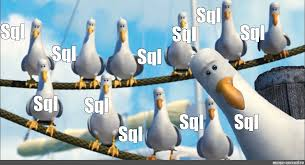
\includegraphics[width=\paperwidth,height=\paperheight]{sql+.jpeg}
	}
	
	\begin{frame}
	\end{frame}
}

%------------------------------------------------

\begin{frame}
	
	\frametitle{Problema}
	
	Supongamos que existe una tabla llamada ``Pedido'' que almacena información sobre los clientes. Cada vez que se inserta un nuevo pedido en esta tabla, también se desea actualizar \textcolor<2>{red}{automáticamente} la tabla ``Inventario'' para reflejar la disminución de existencias de los productos.
	
\end{frame}

%------------------------------------------------

\begin{frame}
	
	\frametitle{Solución}
	
    \centering
    \Huge Disparadores
	
\end{frame}

%------------------------------------------------

\begin{frame}[t]
	
	\frametitle{Características de un disparador (\emph{trigger})}
	
	\begin{itemize}
		
		\item Es un procedimiento que se activa automáticamente sobre una tabla asociada previamente
		
		\pause
		\item Los posibles eventos que activan el \emph{trigger} son aquellas operaciones que modifican el estado de la tabla, o sea: 
			\begin{itemize}
				\item \textcolor{codepurple}{INSERT}
				\item \textcolor{codepurple}{UPDATE}
				\item \textcolor{codepurple}{DELETE}
			\end{itemize}
			
		\pause
		\item No requiere intervención humana o programática para ejecutarse y no se puede detener una vez activado
		
		\pause
		\item Se utiliza para garantizar el cumplimiento de ciertas reglas del negocio y modificar los valores de los atributos de forma dinámica
		
	\end{itemize}	
	
\end{frame}

%------------------------------------------------

\begin{frame}[fragile]
	
	\frametitle{Ventajas de los \emph{triggers}}
	
	Este recurso brindado por SQL permite al programador:
	
	\begin{itemize}
		
		\item Realizar cambios en cascada en la base de datos
		
		\pause 
		
		\item Comprobar restricciones más complejas que las definidas en el \textcolor{codepurple}{CHECK}
		
		\pause
		
		\item Evaluar el estado de una tabla antes y después de realizar una modificación de datos y actuar en función de la diferencia utilizando \textcolor{codepurple}{NEW} y \textcolor{codepurple}{OLD}
		
		\pause
		
		\item Tratar errores de manera más personalizada y compleja
		
	\end{itemize}

\end{frame}

%------------------------------------------------

\begin{frame}[fragile]
	
	\frametitle{Contexto de ejecución de dos \emph{triggers}}
	
	\begin{figure}[h]
		\centering
		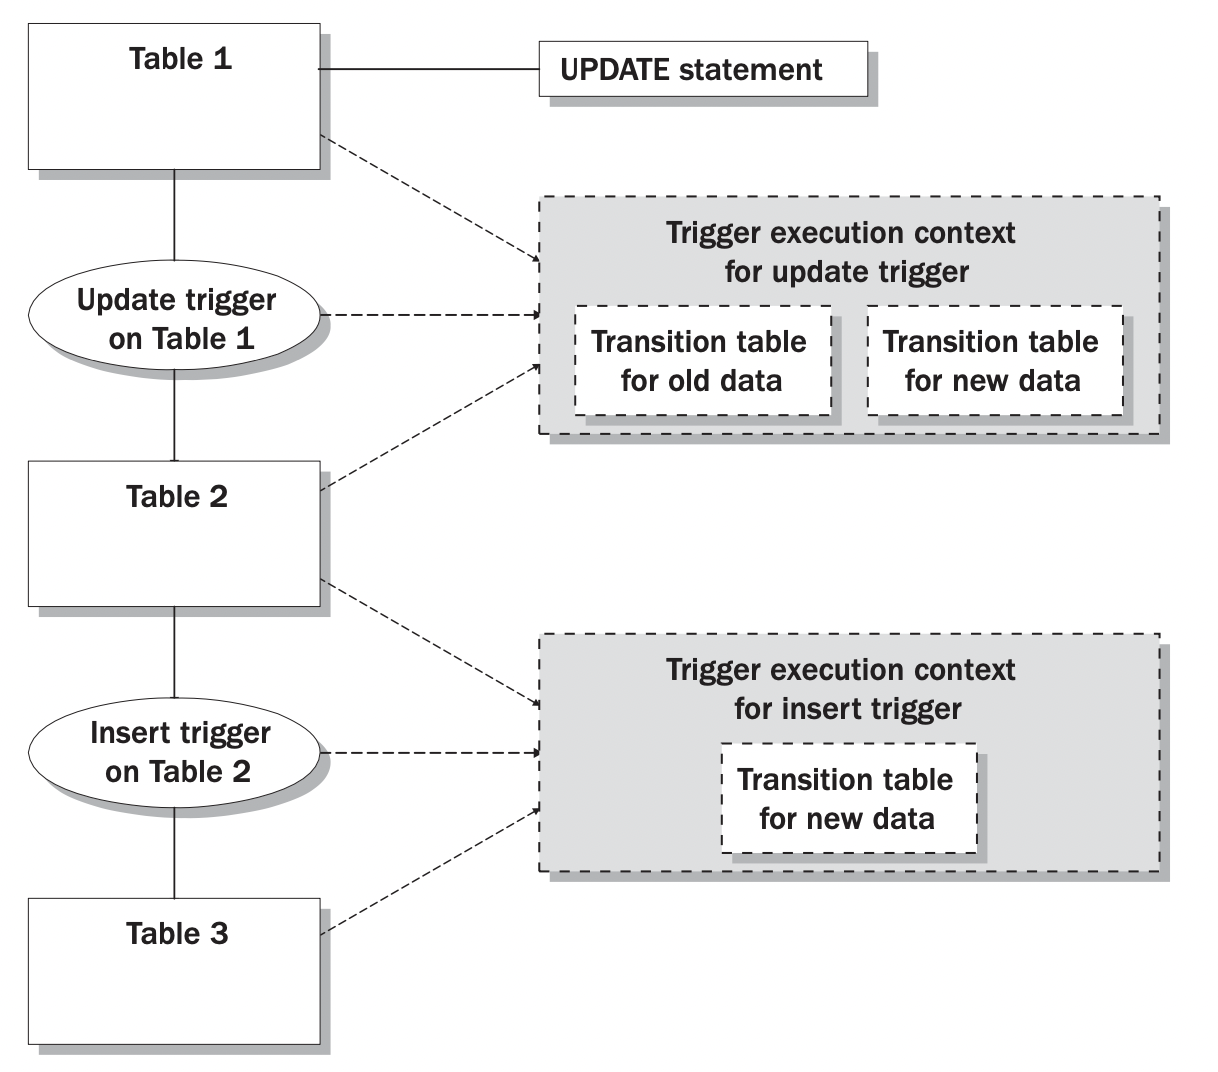
\includegraphics[scale=0.4]{flujo-trigger.png}
	\end{figure}

\end{frame}

%------------------------------------------------

\begin{frame}[fragile]
	
	\frametitle{Sintaxis de los \emph{triggers}}
	
	\begin{lstlisting}[ language=SQL,
		deletekeywords={IDENTITY},
		deletekeywords={[2]INT},
		morekeywords={clustered},
		framesep=8pt,
		xleftmargin=40pt,
		framexleftmargin=40pt,
		frame=tb,
		framerule=0pt ]
CREATE TRIGGER <trigger_name> <trigger_order> <trigger_event> 
ON <table_name> 
FOR EACH ROW <trigger_statement>;
\end{lstlisting}

	\ 
	
	\ 
	
	\pause
	
	El campo \texttt{<trigger\_order>} define el momento en que se ejecuta/activa un \emph{trigger}:
	
	\begin{itemize}
		
		\item \textcolor{codepurple}{BEFORE} 
		\\ Antes de ejecutarse la cláusula definida
		
		\item \textcolor{codepurple}{AFTER} 
		\\ Posterior a la ejecución de la cláusula definida
		
	\end{itemize}
	
\end{frame}

%------------------------------------------------

\begin{frame}[fragile]
	
	\frametitle{Sintaxis de los \emph{triggers}}
	
	\begin{lstlisting}[ language=SQL,
		deletekeywords={IDENTITY},
		deletekeywords={[2]INT},
		morekeywords={clustered},
		framesep=8pt,
		xleftmargin=40pt,
		framexleftmargin=40pt,
		frame=tb,
		framerule=0pt ]
CREATE TRIGGER <trigger_name> <trigger_order> <trigger_event> 
ON <table_name> 
FOR EACH ROW <trigger_statement>;
\end{lstlisting}
	
	\ 
	
	\ 
	
	\pause
	
	El campo \texttt{<trigger\_event>} establece el evento sobre el cual se define el \emph{trigger}. S\'olo pueden definirse cláusulas que modifican el estado de los registros de la base de datos. 
	
	\pause
	
	\begin{table}
		\begin{tabular}{| c | C{5cm} | C{5cm} |}
			\hline
			Evento & Acceso a la variable \textcolor{codepurple}{NEW} & Acceso a la variable \textcolor{codepurple}{OLD} \\ \hline \hline
			\textcolor{codepurple}{INSERT} & Sí, representa la tupla a insertar & No \\ \hline
			\textcolor{codepurple}{DELETE} & No & Sí, representa la tupla antes de eliminarla \\ \hline
			\textcolor{codepurple}{UPDATE} & Sí, representa la tupla después de editarla & Sí, representa la tupla antes de editarla \\ \hline
		\end{tabular}
	\end{table}
	
\end{frame}

%------------------------------------------------

\begin{frame}[fragile]
	
	\frametitle{Sintaxis de los \emph{triggers}}
	
	\begin{lstlisting}[ language=SQL,
		deletekeywords={IDENTITY},
		deletekeywords={[2]INT},
		morekeywords={clustered},
		framesep=8pt,
		xleftmargin=40pt,
		framexleftmargin=40pt,
		frame=tb,
		framerule=0pt ]
CREATE TRIGGER <trigger_name> <trigger_order> <trigger_event> 
ON <table_name> 
FOR EACH ROW <trigger_statement>;
\end{lstlisting}

	\pause
	
	La expresión \texttt{<trigger\_statement>} permite utilizar instrucciones de la programación imperativa y combinarla con las siguientes instrucciones declarativas: 
	\begin{columns}[t]
		\column{0.3\textwidth}
		
		\begin{itemize}
			\item \textcolor{codepurple}{INSERT}
			\item \textcolor{codepurple}{UPDATE}
			\item \textcolor{codepurple}{DELETE}
		\end{itemize}
		
		\column{0.3\textwidth}
		
		\begin{itemize}
			\item \textcolor{codepurple}{CREATE}
			\item \textcolor{codepurple}{DROP}
			\item \textcolor{codepurple}{ALTER}
		\end{itemize}
		
		\column{0.3\textwidth}
		
		\begin{itemize}
			\item \textcolor{codepurple}{SELECT}
		\end{itemize}
		
	\end{columns}
	
	\ 
	
	\ 
	
	\pause
	
	Estructura: 
		\begin{lstlisting}[ language=SQL,
		deletekeywords={IDENTITY},
		deletekeywords={[2]INT},
		morekeywords={clustered},
		framesep=8pt,
		xleftmargin=40pt,
		framexleftmargin=40pt,
		frame=tb,
		framerule=0pt ]
BEGIN
<body>
END;
\end{lstlisting}
	
\end{frame}

%------------------------------------------------

\begin{frame}[fragile]
	
	\frametitle{Algunas instrucciones imperativas}
	
	\begin{columns}[t]
		\column{0.5\textwidth}
		
			\begin{itemize}
			
			\item Declaración de variables \\
			\texttt{\textcolor{codepurple}{DECLARE} <var\_name> <var\_type>} \\ 
			\texttt{\textcolor{codepurple}{@}<var\_name>}
			
			\pause
			\ 
			
			\item  Asignación de valor \\ 
			\texttt{\textcolor{codepurple}{SET} <var\_name> = <value>}
			
			\pause
			\ 
			
			\item  Uso de condiciones \\
			\texttt{\textcolor{codepurple}{IF} <conditional\_expression> \\ 
				\textcolor{codepurple}{THEN} <statements\_block> \\ 
				\textcolor{codepurple}{ELSE} <statements\_block> \\ 
				\textcolor{codepurple}{END IF}}
			
		\end{itemize}
		
		\column{0.5\textwidth}
		
			\begin{itemize}
				
			\pause 
						
			\item Uso de ciclos (WHILE / DO-WHILE)\\
			\texttt{\textcolor{codepurple}{WHILE}  <conditional\_expression>  \\
			\textcolor{codepurple}{DO}  <statements\_block> \\
			\textcolor{codepurple}{END WHILE}} \\
			
			\ 
			
			\texttt{\textcolor{codepurple}{REPEAT}  <statements\_block>  \\
			\textcolor{codepurple}{UNTIL} <conditional\_expression> \\
			\textcolor{codepurple}{END REPEAT}}
			
			\pause
			\ 
			
			\item Detener ciclos (BREAK)\\ 
			\texttt{\textcolor{codepurple}{LEAVE}}
			
		\end{itemize}
		
	\end{columns}
	
\end{frame}

%------------------------------------------------

\begin{frame}{t}
	
	\frametitle{Recordando nuestra base de datos}
	
	\begin{figure}[h]
		\centering
		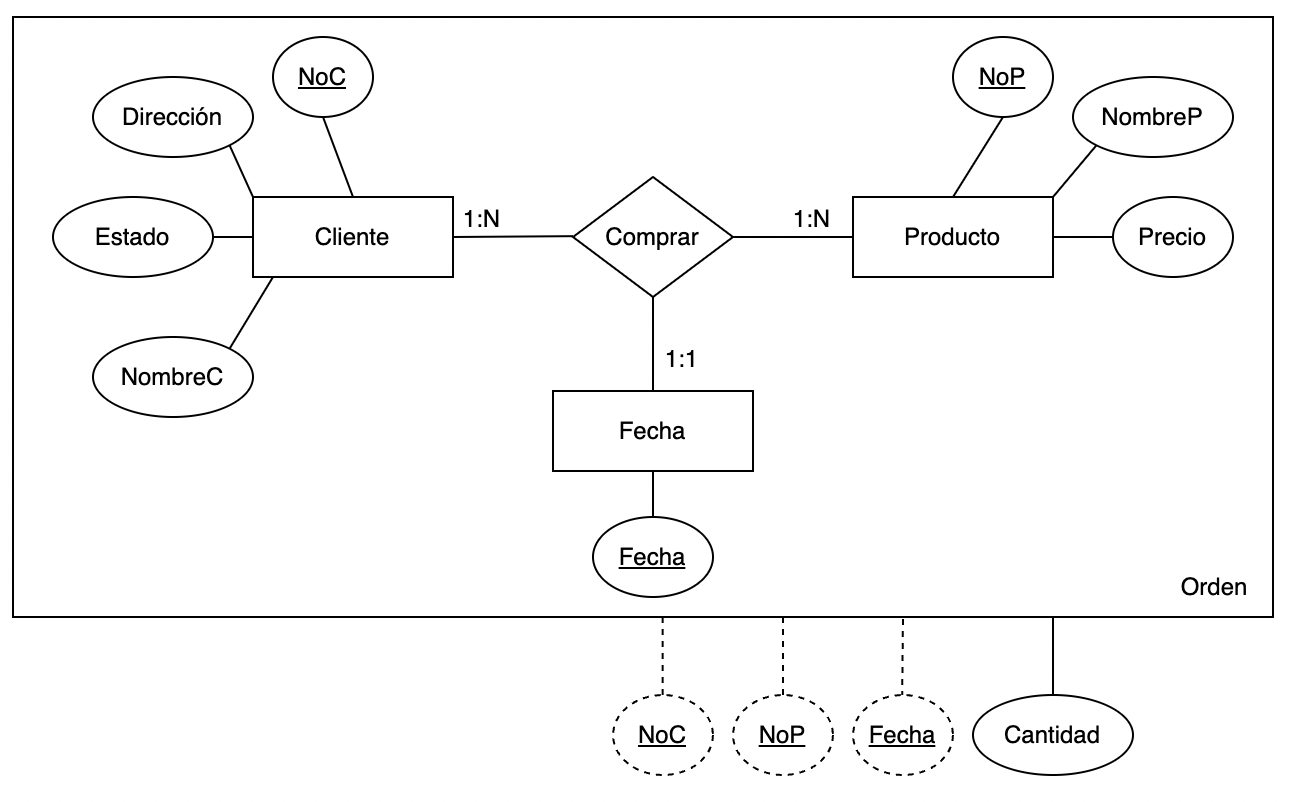
\includegraphics[scale=0.5]{bd.png}
	\end{figure}
	
	
\end{frame}

%------------------------------------------------

\begin{frame}[fragile]
	
	\frametitle{Ejemplo}
	
	Problema: \\
	Construya un \emph{trigger} para limitar la cantidad de unidades por producto, en una orden de compra. Cada producto tiene definido el máximo de compras por día.
	
	\ 
	
	Solución: \\
	
	\begin{onlyenv}<1-2>
		\begin{lstlisting}[ language=SQL,
			deletekeywords={IDENTITY},
			deletekeywords={[2]INT},
			morekeywords={clustered},
			framesep=8pt,
			xleftmargin=40pt,
			framexleftmargin=40pt,
			frame=tb,
			framerule=0pt ]
CREATE TRIGGER trg_limit_test <trigger_order> <trigger_event> 
ON <table_name> 
FOR EACH ROW <trigger_statement>;
\end{lstlisting}
	\end{onlyenv}

	\begin{onlyenv}<3-4>
		\begin{lstlisting}[ language=SQL,
			deletekeywords={IDENTITY},
			deletekeywords={[2]INT},
			morekeywords={clustered},
			framesep=8pt,
			xleftmargin=40pt,
			framexleftmargin=40pt,
			frame=tb,
			framerule=0pt ]
CREATE TRIGGER <trigger_name> <trigger_order> <trigger_event> 
ON Orden
FOR EACH ROW <trigger_statement>;
\end{lstlisting}
	\end{onlyenv}
	
	\begin{onlyenv}<5-6>
		\begin{lstlisting}[ language=SQL,
			deletekeywords={IDENTITY},
			deletekeywords={[2]INT},
			morekeywords={clustered},
			framesep=8pt,
			xleftmargin=40pt,
			framexleftmargin=40pt,
			frame=tb,
			framerule=0pt ]
CREATE TRIGGER <trigger_name> BEFORE INSERT 
ON orden
FOR EACH ROW <trigger_statement>;
\end{lstlisting}
	\end{onlyenv}
	
		\begin{onlyenv}<7>
		\begin{lstlisting}[ language=SQL,
			deletekeywords={IDENTITY},
			deletekeywords={[2]INT},
			morekeywords={clustered},
			framesep=8pt,
			xleftmargin=40pt,
			framexleftmargin=40pt,
			frame=tb,
			framerule=0pt ]
CREATE TRIGGER <trigger_name> BEFORE INSERT 
ON Orden FOR EACH ROW 
BEGIN
  -- (1) Dado el cliente (NEW.NoC), obtener la cantidad de productos igual al comprado (NEW.NoP), adquiridos en la fecha actual (NEW.Fecha)
  
  -- (2) Obtener el límite de productos del tipo NEW.NoP, que se puede adquirir en un mismo día
  
  -- (3) Verificar si la cantidad de productos comprados, más la almacenada, supera la cantidad límite
END;
\end{lstlisting}
\end{onlyenv}
		
	\ 
	
	\ 
	
	\only<2>{\textcolor{red}{¿Sobre qué relación trabajará el \emph{trigger}?}}
	
	\only<4>{\textcolor{red}{¿Con el uso de qué clásula se activará el \emph{trigger}? ¿Cuándo lo hará?}}
	
	\only<6>{\textcolor{red}{¿Qué debe de hacer el \emph{trigger}?}}
	
\end{frame}

%------------------------------------------------

\begin{frame}[fragile]
	
	\frametitle{Ejemplo - Solución}
	
	\begin{lstlisting}[ language=SQL,
		deletekeywords={IDENTITY},
		deletekeywords={[2]INT},
		morekeywords={clustered},
		framesep=8pt,
		xleftmargin=40pt,
		framexleftmargin=40pt,
		frame=tb,
		framerule=0pt ]
CREATE TRIGGER trg_limit_test BEFORE INSERT ON Orden 
FOR EACH ROW BEGIN
  DECLARE total INT;
  DECLARE limiteDiario INT;
  SET total = (-- (1) 
    SELECT SUM(Cantidad) 
    FROM orden 
    WHERE NoC = NEW.NoC AND NoP = NEW.NoP AND DATE(Fecha) = DATE(NEW.Fecha)
  );-- (2)
  SET limiteDiario = (
    SELECT MIN(producto.LimiteDiario) 
    FROM producto 
    WHERE producto.NoP = NEW.NoP
  );-- (3)
  IF total + NEW.Cantidad > limiteDiario THEN
    SIGNAL SQLSTATE '45000' SET MESSAGE_TEXT = 'Acaparador!!!';
  END IF;
END;
\end{lstlisting}

\end{frame}

%------------------------------------------------

\begin{frame}{t}
	
	\frametitle{Algunas restricciones de los \emph{triggers}}
	
	\begin{itemize}
		
		\item No recibe parámetros de entrada o salida
		
		\pause
		
		\item La única forma de trabajar con la fila ``modificada'' es a través de las pseudovariables (\textcolor{codepurple}{NEW} y \textcolor{codepurple}{OLD})
		
		\pause
		
		\item No se puede ejecutar una operación de modificación sobre la misma tabla donde el \emph{trigger} se define
		
		\pause
		
		\item No se puede ejecutar una tarea sobre otra tabla, si la segunda tiene un \emph{trigger} que afecte a la tabla del primer \emph{trigger} en ejecución, o sea, no se acepta recursividad
		
		\pause
		
		\item No se puede invocar desde un \emph{trigger} procedimientos con parámetros \textcolor{codepurple}{OUT} o \textcolor{codepurple}{INOUT} o que trabaje con SQL dinámico.
		
	\end{itemize}
	
\end{frame}
